\textcolor{\mycolor}{
From experimental point of view, the process cross section can be determined applying generic formula:
\begin{equation}
\sigma = \left(N_{\mathrm{sig}}-N_{\mathrm{bg}}\right)\cdot \mathcal{A} \cdot \mathcal{L}^{-1},
\label{eq:csdef}
\end{equation}
where $N_{\mathrm{sig}}\left(N_{\mathrm{bg}}\right)$, denotes an estimate of the number of signal (background) events, while $\mathcal{L}$ and $\mathcal{A}$ represent an integrated luminosity and a correction factor taking detector and possibly other effects into account, respectively. }

\textcolor{\mycolor}{
As follows from the Eq.~\eqref{eq:csdef}, to measure the process cross section, typically several steps have to be performed, i.e. the number of signal and background events as well as the integrated luminosity have to be determined for a given data sample; the detector effects attributed to e.g. inefficiencies, finite resolution, etc. also have to be taken into account. On the other hand, in the direct searchers for new phenomena, typically the regions of phase space are investigated in which the signal production cross section is enhanced and exceeds the background significantly. In general, in this procedure certain assumptions about e.g. modelling of the detector response or the shape of the background spectrum are typically made. The sensitivity of the result to variations of different assumptions is called systematic uncertainty and is one of the crucial components of the analysis that often requires elaborate studies. Besides that, the precision of the measurements with low event count rate as e.g. \fourtop production, is usually limited by stochastic effects\footnote{Typically attributed to statistical uncertainty on the number of signal events.}, which also have to be properly taken into account. To achieve all mentioned tasks, various techniques, employing simulations of relevant processes, data-driven analysis methods and statistical means, exist. The proposed research follows closely well established paradigm in the field. The foreseen steps and intermediate goals of this study are detailed below.}

\textcolor{\mycolor}{
Depending on the principal task, i.e. measurement of the SM cross section or direct search for BSM signal, two corresponding sub-projects can be identified in this proposal. In general, any experimental analysis aims at best measurement precision, however, in case of searches for new phenomena, the maximal statistical significance of the signal is required in addition.
% The $b$- and $t$-reconstruction and tagging algorithms, to be described below, are being developed in order to minimise background contamination, $N_{\mathrm{bg}}$, and to reconstruct maximum possible number of signal events, $N_{\mathrm{sig}}$ in case of direct searches, and to be maximally robust against detector effects in case of cross section measurement. As follows from Eq.~\ref{eq:csdef}, 
%
Two different strategies will be pursued in the respective sub-projects, however both can be performed using comparable tools. Furthermore, it is natural to split the sub-projects further according to the $t\bar{t}t\bar{t}$ decay channel to be considered, corresponding to zero-, single- and two-lepton final states, respectively. As all three have different experimental signatures, development and optimisation of individual reconstruction algorithms, selection of appropriate trigger chains, background studies as well as determination of statistical and systematic effects will be different in three sub-projects. However, they have a common core related to the reconstruction and identification of $b$-quark jets and reconstruction of hadronic top decays.}

\textcolor{\mycolor}{The single-lepton channel, for which I was the lead author of~\cite{Sirunyan:2017tep} and the VUB group worked on in~\cite{Khachatryan:2014sca} is considered the most straight-forward analysis in this project. It has the largest branching fraction and expected to have moderate and well-understood background. Moreover, constrained-kinematics reconstruction, extensively employed in CMS in top-pair production analyses at the VUB, is directly applicable in this channel and will have significant effect on top quark identification efficiency. This sub-project will largely benefit from my extensive experience in this analysis and will use state-of-the-art dedicated tools developed at the host institution.
\begin{figure}
\centering
\begin{subfigure}[t]{0.5\textwidth}
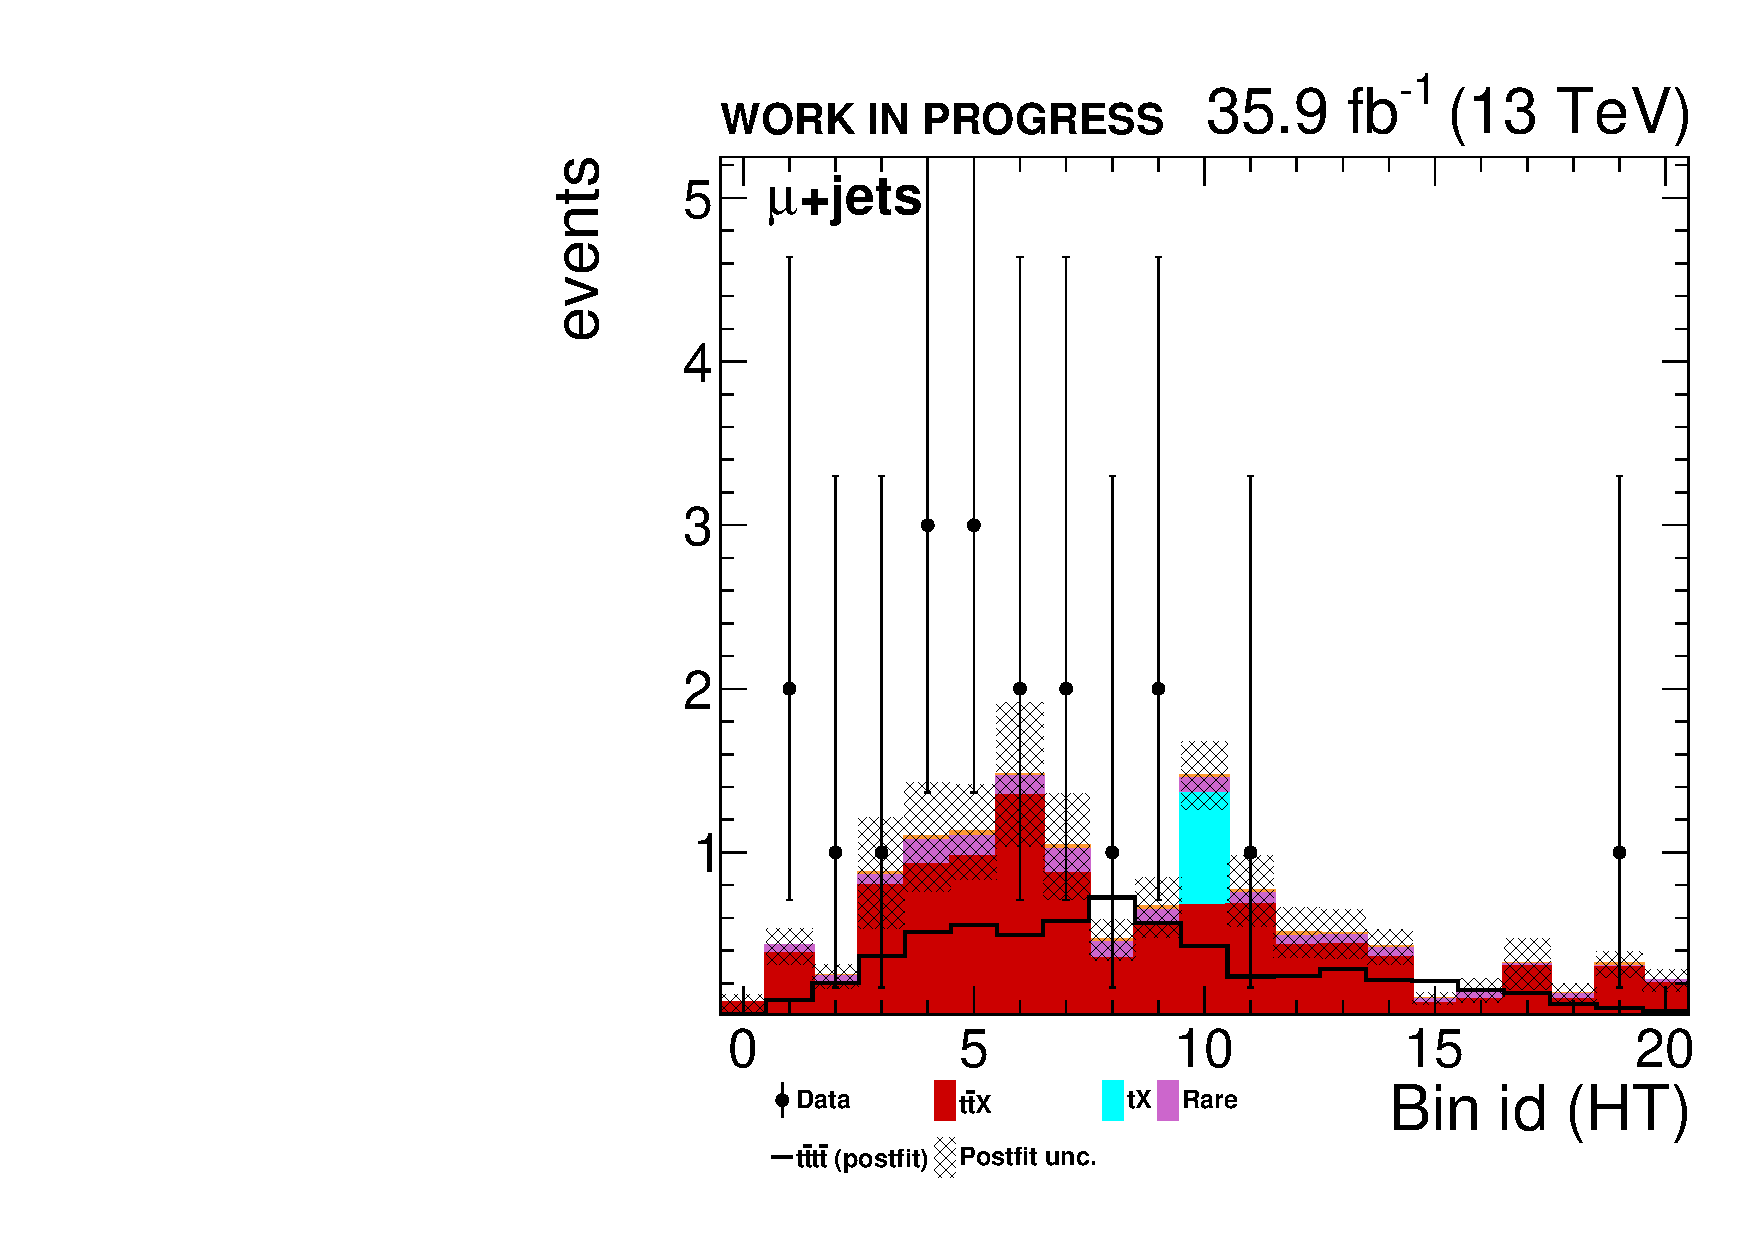
\includegraphics[width=0.8\linewidth]{figures/mu_ht_lin}\subcaption{}\label{fig:2a}
\end{subfigure}%
\begin{subfigure}[t]{0.5\textwidth}
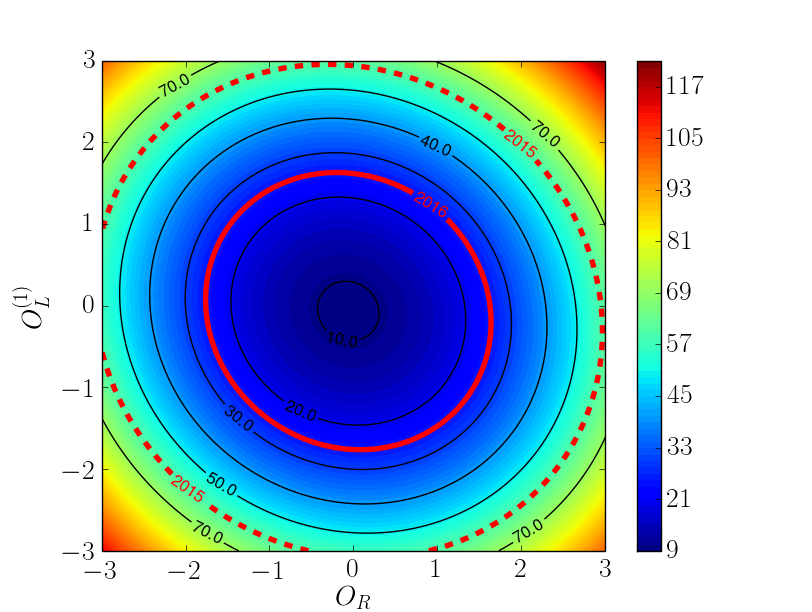
\includegraphics[width=\linewidth]{figures/C1_C2}\subcaption{}\label{fig:2b}
\end{subfigure}%
\caption{\textbf{Work in progress.} (a) Distribution of scalar sum of transverse momenta of hadronic jets, $\mathrm{HT}$, in the most sensitive search region (10 jets and 4 b tags) in $\mu+$jets channel obtained using 35.9 \invfb dataset collected during 2016 data tacking period. Observations are shown as black dots, while background predictions obtained from Monte Carlo simulations are shown as a stacked histogram. Uncertainties on MC predictions obtained from the fit to the data in control regions are shown as hatched area. (b) Independent limits on four fermion dimension 6 operators $O_{L}^{\left(1 \right) }$ and $O_R$, defined in~\cite{DegrandeEFTthesis} (see also ~\cite{Zhang:2017mls}), that can be obtained using 2015 (dashed line) or 2016 (solid line) datasets. The region outside red dashed or solid ellipses are excluded by observations. Color axis represents predictions for four top total cross section, $\sigma_{t\bar{t}t\bar{t}}$, for given values of effective coupling parameters (Wilson coefficients) of $O_{L}^{\left(1 \right) }$ and $O_R$ operators. }
\label{fig:mu}
\end{figure}
The CMS collaboration already has published results obtained in same-sign dilepton and multilepton channels~\cite{Sirunyan:2017roi} based on the same dataset, and this analysis observes a 1.6 $\sigma$ excess. This proposal focuses on the complementary lepton+jets final state. The analysis framework for event selection and resolved hadronic top decays reconstruction was already developed by the applicant and interfaced with statistical interpretation software. Initial results that were obtained using 35.9 \invfb of integrated luminosity collected in 2016 are still under investigation within the CMS collaboration and are shown in Fig.~\ref{fig:2a} (for review purposes only). It demonstrates the distribution of $HT$ in the most sensitive search region. First studies indicate that there may be an excess of signal over SM predictions, but further investigation will be necessary to understand the nature of observed distributions. The single-lepton channel will be important to claim or disprove a first hint of \tttt production at this early stage, while for larger datasets and all channels will be necessary to claim an observation. \textbf{It will be crucial to analyse the 2016--2018 data in the lepton+jets channel to confirm if the 1.6 $\sigma$ excess observed in ~\cite{Sirunyan:2017roi} is a statistical fluctuation or the first hint of a signal, possibly at larger cross sections than the current best SM predictions.} In general, the direct search for \tttt production in this channel represents the minimal goal of the proposal. The results of this study using 2016 and 2017 data are already novel enough to be independently published in peer-reviewed journals. }

\textcolor{\mycolor}{
To complete the analysis and draw the conclusions about the impact of new searches, the data can be interpreted within the so-called effective-field theory (EFT) approach in which the impact of BSM physics is parametrised by higher-dimensional operators constructed from the products of SM fields. In my opinion, this is the optimal approach, because these results, in contrast to a particular ultraviolet-complete model, have much broader scope and, at least in principle, can be reinterpreted within any BSM model. The EFT-analysis of the measurements is a novel approach to the interpretation of the $t\bar{t}t\bar{t}$ data and may attract larger attention to the obtained results. The outcome of this analysis can be presented as a \textbf{separate publication} or together with the results of the searches. }

\textcolor{\mycolor}{
Preliminary research on EFT interpretation has been already carried out in the context of a Bachelor thesis where the applicant was co-promotor. This study will be modified to be applicable to the 2016 data analysis. As an example, Fig.~\ref{fig:2b} demonstrates the comparison of constrains on dimension-6 four-fermion operators contributing to four top quarks production at the LHC that was obtained by the applicant (see also Bsc. thesis~\cite{MathiasThesis} for analysis of 2015 data). As can be seen, significant improvement can be achieved with larger Run 2 data sample. Even stronger constraints, potentially ruling out some theoretical models, can be obtained with the full Run 2 dataset.
}

\textcolor{\mycolor}{
Determination of the $t\bar{t}t\bar{t}$ production cross section in other channels and corresponding searches are a logical extension of the described analysis. The two-lepton channel can provide a valuable contribution with a moderate effort, while the analysis in the zero-lepton channel may present significant challenge due to major difference in the final-state. In order to reach the ultimate sensitivity in the BSM searches, the next logical step, contingent with these sub-tasks, is a combination and interpretation of the results obtained in various channels. They will perfectly fit together with the analysis of the single-lepton channel, but can be issued together with the combination in a \textbf{separate publication}. \textbf{My experience in four top searches makes me perfect candidate for all these tasks.}}

\textcolor{\mycolor}{
To fulfil the ambitious plans outlined above, the research will be delivered in several work-packages which are elucidated in the following.}
% baseline selection and event reconstruction
% interpretation of the results within specific and EFT models. Cite Chen:2014ewl
